\documentclass[12pt,twoside]{article}

\newcommand{\reporttitle}{Project 3: Collaboration and Competition}
\newcommand{\reportauthor}{Thomas Teh}
\newcommand{\reporttype}{Project Report}
\newcommand{\cid}{0124 3008}

% include files that load packages and define macros
%%%%%%%%%%%%%%%%%%%%%%%%%%%%%%%%%%%%%%%%%
% University Assignment Title Page 
% LaTeX Template
% Version 1.0 (27/12/12)
%
% This template has been downloaded from:
% http://www.LaTeXTemplates.com
%
% Original author:
% WikiBooks (http://en.wikibooks.org/wiki/LaTeX/Title_Creation)
%
% License:
% CC BY-NC-SA 3.0 (http://creativecommons.org/licenses/by-nc-sa/3.0/)
% 
% Instructions for using this template:
% This title page is capable of being compiled as is. This is not useful for 
% including it in another document. To do this, you have two options: 
%
% 1) Copy/paste everything between \begin{document} and \end{document} 
% starting at \begin{titlepage} and paste this into another LaTeX file where you 
% want your title page.
% OR
% 2) Remove everything outside the \begin{titlepage} and \end{titlepage} and 
% move this file to the same directory as the LaTeX file you wish to add it to. 
% Then add \input{./title_page_1.tex} to your LaTeX file where you want your
% title page.
%
%----------------------------------------------------------------------------------------
%	PACKAGES AND OTHER DOCUMENT CONFIGURATIONS
%----------------------------------------------------------------------------------------
\usepackage{ifxetex}
\usepackage{textpos}
%\usepackage{natbib}
%\usepackage{breqn}
\usepackage{kpfonts}
\usepackage[a4paper,hmargin=2.8cm,vmargin=2.0cm,includeheadfoot]{geometry}
\usepackage{ifxetex}
\usepackage{stackengine}
\usepackage{tabularx,longtable,multirow,subfigure,caption}%hangcaption
\usepackage{fncylab} %formatting of labels
\usepackage{fancyhdr}
\usepackage{color}
\usepackage[tight,ugly]{units}
\usepackage{url}
\usepackage{float}
\usepackage[english]{babel}
\usepackage{amsmath}
\usepackage{graphicx}
\usepackage[colorinlistoftodos]{todonotes}
\usepackage{dsfont}
\usepackage{epstopdf} % automatically replace .eps with .pdf in graphics
\usepackage{natbib}
\usepackage{backref}
\usepackage{array}
\usepackage{latexsym}
\usepackage{etoolbox}
\usepackage{algorithmic}
\usepackage[]{algorithm2e}

\usepackage{enumerate} % for numbering with [a)] format 



\ifxetex
\usepackage{fontspec}
\setmainfont[Scale=.8]{OpenDyslexic-Regular}
\else
\usepackage[pdftex,pagebackref,hypertexnames=false,colorlinks]{hyperref} % provide links in pdf
\hypersetup{pdftitle={},
  pdfsubject={}, 
  pdfauthor={\reportauthor},
  pdfkeywords={}, 
  pdfstartview=FitH,
  pdfpagemode={UseOutlines},% None, FullScreen, UseOutlines
  bookmarksnumbered=true, bookmarksopen=true, colorlinks,
    citecolor=black,%
    filecolor=black,%
    linkcolor=black,%
    urlcolor=black}
\usepackage[all]{hypcap}
\fi

\usepackage{tcolorbox}

% various theorems
\usepackage{ntheorem}
\theoremstyle{break}
\newtheorem{lemma}{Lemma}
\newtheorem{theorem}{Theorem}
\newtheorem{remark}{Remark}
\newtheorem{definition}{Definition}
\newtheorem{proof}{Proof}

% example-environment
\newenvironment{example}[1][]
{ 
\vspace{4mm}
\noindent\makebox[\linewidth]{\rule{\hsize}{1.5pt}}
\textbf{Example #1}\\
}
{ 
\noindent\newline\makebox[\linewidth]{\rule{\hsize}{1.0pt}}
}



%\renewcommand{\rmdefault}{pplx} % Palatino
% \renewcommand{\rmdefault}{put} % Utopia

\ifxetex
\else
\renewcommand*{\rmdefault}{bch} % Charter
\renewcommand*{\ttdefault}{cmtt} % Computer Modern Typewriter
%\renewcommand*{\rmdefault}{phv} % Helvetica
%\renewcommand*{\rmdefault}{iwona} % Avant Garde
\fi

\setlength{\parindent}{0em}  % indentation of paragraph

\setlength{\headheight}{14.5pt}
\pagestyle{fancy}
\fancyfoot[ER,OL]{\thepage}%Page no. in the left on
                                %odd pages and on right on even pages
\fancyfoot[OC,EC]{\sffamily }
\renewcommand{\headrulewidth}{0.1pt}
\renewcommand{\footrulewidth}{0.1pt}
\captionsetup{margin=10pt,font=small,labelfont=bf}


%--- chapter heading

\def\@makechapterhead#1{%
  \vspace*{10\p@}%
  {\parindent \z@ \raggedright %\sffamily
        %{\Large \MakeUppercase{\@chapapp} \space \thechapter}
        %\\
        %\hrulefill
        %\par\nobreak
        %\vskip 10\p@
    \interlinepenalty\@M
    \Huge \bfseries 
    \thechapter \space\space #1\par\nobreak
    \vskip 30\p@
  }}

%---chapter heading for \chapter*  
\def\@makeschapterhead#1{%
  \vspace*{10\p@}%
  {\parindent \z@ \raggedright
    \sffamily
    \interlinepenalty\@M
    \Huge \bfseries  
    #1\par\nobreak
    \vskip 30\p@
  }}
  



% %%%%%%%%%%%%% boxit
\def\Beginboxit
   {\par
    \vbox\bgroup
	   \hrule
	   \hbox\bgroup
		  \vrule \kern1.2pt %
		  \vbox\bgroup\kern1.2pt
   }

\def\Endboxit{%
			      \kern1.2pt
		       \egroup
		  \kern1.2pt\vrule
		\egroup
	   \hrule
	 \egroup
   }	

\newenvironment{boxit}{\Beginboxit}{\Endboxit}
\newenvironment{boxit*}{\Beginboxit\hbox to\hsize{}}{\Endboxit}



\allowdisplaybreaks

\makeatletter
\newcounter{elimination@steps}
\newcolumntype{R}[1]{>{\raggedleft\arraybackslash$}p{#1}<{$}}
\def\elimination@num@rights{}
\def\elimination@num@variables{}
\def\elimination@col@width{}
\newenvironment{elimination}[4][0]
{
    \setcounter{elimination@steps}{0}
    \def\elimination@num@rights{#1}
    \def\elimination@num@variables{#2}
    \def\elimination@col@width{#3}
    \renewcommand{\arraystretch}{#4}
    \start@align\@ne\st@rredtrue\m@ne
}
{
    \endalign
    \ignorespacesafterend
}
\newcommand{\eliminationstep}[2]
{
    \ifnum\value{elimination@steps}>0\leadsto\quad\fi
    \left[
        \ifnum\elimination@num@rights>0
            \begin{array}
            {@{}*{\elimination@num@variables}{R{\elimination@col@width}}
            |@{}*{\elimination@num@rights}{R{\elimination@col@width}}}
        \else
            \begin{array}
            {@{}*{\elimination@num@variables}{R{\elimination@col@width}}}
        \fi
            #1
        \end{array}
    \right]
    & 
    \begin{array}{l}
        #2
    \end{array}
    &%                                    moved second & here
    \addtocounter{elimination@steps}{1}
}
\makeatother

%% Fast macro for column vectors
\makeatletter  
\def\colvec#1{\expandafter\colvec@i#1,,,,,,,,,\@nil}
\def\colvec@i#1,#2,#3,#4,#5,#6,#7,#8,#9\@nil{% 
  \ifx$#2$ \begin{bmatrix}#1\end{bmatrix} \else
    \ifx$#3$ \begin{bmatrix}#1\\#2\end{bmatrix} \else
      \ifx$#4$ \begin{bmatrix}#1\\#2\\#3\end{bmatrix}\else
        \ifx$#5$ \begin{bmatrix}#1\\#2\\#3\\#4\end{bmatrix}\else
          \ifx$#6$ \begin{bmatrix}#1\\#2\\#3\\#4\\#5\end{bmatrix}\else
            \ifx$#7$ \begin{bmatrix}#1\\#2\\#3\\#4\\#5\\#6\end{bmatrix}\else
              \ifx$#8$ \begin{bmatrix}#1\\#2\\#3\\#4\\#5\\#6\\#7\end{bmatrix}\else
                 \PackageError{Column Vector}{The vector you tried to write is too big, use bmatrix instead}{Try using the bmatrix environment}
              \fi
            \fi
          \fi
        \fi
      \fi
    \fi
  \fi 
}  
\makeatother

\robustify{\colvec}

%%% Local Variables: 
%%% mode: latex
%%% TeX-master: "notes"
%%% End: 
 % various packages needed for maths etc.
% quick way of adding a figure
\newcommand{\fig}[3]{
 \begin{center}
 \scalebox{#3}{\includegraphics[#2]{#1}}
 \end{center}
}

%\newcommand*{\point}[1]{\vec{\mkern0mu#1}}
\newcommand{\ci}[0]{\perp\!\!\!\!\!\perp} % conditional independence
\newcommand{\point}[1]{{#1}} % points 
\renewcommand{\vec}[1]{{\boldsymbol{{#1}}}} % vector
\newcommand{\mat}[1]{{\boldsymbol{{#1}}}} % matrix
\newcommand{\R}[0]{\mathds{R}} % real numbers
\newcommand{\Z}[0]{\mathds{Z}} % integers
\newcommand{\N}[0]{\mathds{N}} % natural numbers
\newcommand{\nat}[0]{\mathds{N}} % natural numbers
\newcommand{\Q}[0]{\mathds{Q}} % rational numbers
\ifxetex
\newcommand{\C}[0]{\mathds{C}} % complex numbers
\else
\newcommand{\C}[0]{\mathds{C}} % complex numbers
\fi
\newcommand{\tr}[0]{\text{tr}} % trace
\renewcommand{\d}[0]{\mathrm{d}} % total derivative
\newcommand{\inv}{^{-1}} % inverse
\newcommand{\id}{\mathrm{id}} % identity mapping
\renewcommand{\dim}{\mathrm{dim}} % dimension
\newcommand{\rank}[0]{\mathrm{rk}} % rank
\newcommand{\determ}[1]{\mathrm{det}(#1)} % determinant
\newcommand{\scp}[2]{\langle #1 , #2 \rangle}
\newcommand{\kernel}[0]{\mathrm{ker}} % kernel/nullspace
\newcommand{\img}[0]{\mathrm{Im}} % image
\newcommand{\idx}[1]{{(#1)}}
\DeclareMathOperator*{\diag}{diag}
\newcommand{\E}{\mathds{E}} % expectation
\newcommand{\var}{\mathds{V}} % variance
\newcommand{\gauss}[2]{\mathcal{N}\big(#1,\,#2\big)} % gaussian distribution N(.,.)
\newcommand{\gaussx}[3]{\mathcal{N}\big(#1\,|\,#2,\,#3\big)} % gaussian distribution N(.|.,.)
\newcommand{\gaussBig}[2]{\mathcal{N}\left(#1,\,#2\right)} % see above, but with brackets that adjust to the height of the arguments
\newcommand{\gaussxBig}[3]{\mathcal{N}\left(#1\,|\,#2,\,#3\right)} % see above, but with brackets that adjust to the height of the arguments
\DeclareMathOperator{\cov}{Cov} % covariance (matrix) 
\ifxetex
\renewcommand{\T}[0]{^\top} % transpose
\else
\newcommand{\T}[0]{^\top}
\fi
% matrix determinant
\newcommand{\matdet}[1]{
\left|
\begin{matrix}
#1
\end{matrix}
\right|
}



%%% various color definitions
\definecolor{darkgreen}{rgb}{0,0.6,0}

\newcommand{\blue}[1]{{\color{blue}#1}}
\newcommand{\red}[1]{{\color{red}#1}}
\newcommand{\green}[1]{{\color{darkgreen}#1}}
\newcommand{\orange}[1]{{\color{orange}#1}}
\newcommand{\magenta}[1]{{\color{magenta}#1}}
\newcommand{\cyan}[1]{{\color{cyan}#1}}


% redefine emph
\renewcommand{\emph}[1]{\blue{\bf{#1}}}

% place a colored box around a character
\gdef\colchar#1#2{%
  \tikz[baseline]{%
  \node[anchor=base,inner sep=2pt,outer sep=0pt,fill = #2!20] {#1};
    }%
}%
 % short-hand notation and macros
\DontPrintSemicolon

%%%%%%%%%%%%%%%%%%%%%%%%%%%%

\begin{document}
% front page
% Last modification: 2016-09-29 (Marc Deisenroth)
\begin{titlepage}

\newcommand{\HRule}{\rule{\linewidth}{0.5mm}} % Defines a new command for the horizontal lines, change thickness here


%----------------------------------------------------------------------------------------
%	LOGO SECTION
%----------------------------------------------------------------------------------------

%
\includegraphics[width = 4cm]{./figures/imperial}\\[0.5cm] 

\begin{center} % Center remainder of the page

%----------------------------------------------------------------------------------------
%	HEADING SECTIONS
%----------------------------------------------------------------------------------------
\textsc{\LARGE \reporttype}\\[1.5cm] 
\textsc{\Large Udacity}\\[0.5cm] 
\textsc{\large Deep Reinforcement Learning Nanodegree}\\[0.5cm] 
%----------------------------------------------------------------------------------------
%	TITLE SECTION
%----------------------------------------------------------------------------------------

\HRule \\[0.4cm]
{ \huge \bfseries \reporttitle}\\ % Title of your document
\HRule \\[1.5cm]
\end{center}
%----------------------------------------------------------------------------------------
%	AUTHOR SECTION
%----------------------------------------------------------------------------------------

%\begin{minipage}{0.4\hsize}
\begin{flushleft} \large
\textsc{Author:}\\
\reportauthor~%(CID: \cid) % Your name
\end{flushleft}
\vspace{2cm}
\makeatletter
Date: \@date 

\vfill % Fill the rest of the page with whitespace



\makeatother


\end{titlepage}




%%%%%%%%%%%%%%%%%%%%%%%%%%%% Main document
\section{Multi-Agent DDPG}
In this project, I tackled the Unity Tennis environment using a multi-agent deep reinforcement framework. The tasks of the agents are to keep the ball within bounds and up in the air as long as possible. Under the multi-agent setting, the two agents that interact with each other are DDPG agents (see \ref{appendix}). 

It is important to note that the interaction between the agents are neither cooperative nor competitive following reasons:
\begin{itemize}
	\item The agents do not have incentives to outperform each other in terms of scores.
	\item The agents do not formulate a shared strategy to keep the ball in play as long as possible.
\end{itemize}

Each agent chooses an action that maximizes the rewards independently, but their objectives are such that it results in cooperative play. When one agent successfully keeps the ball in play, the other agent benefits by having the opportunity to increase its reward by also keeping the ball in play.


\section{The MADDPG Architecture}
The MADDPF architecture was introduced by \citep{lowe2017multi} as shown in Figure \ref{fig:madpgg_architecture}. While the algorithm utilizes the DPPG algorithm for each agent, it is important to note that the actor networks for each agent takes in observations of that particular agent as input. The actor networks of the other agents do not have access to those observations. \\

However, the critic networks of the agents have access to the observations and actions of \textbf{all} agents as inputs. All the agents will contribute to the experience replay buffer and this will allow the agents to learn from one another's experiences.

\begin{figure}[H]
	\begin{center}
		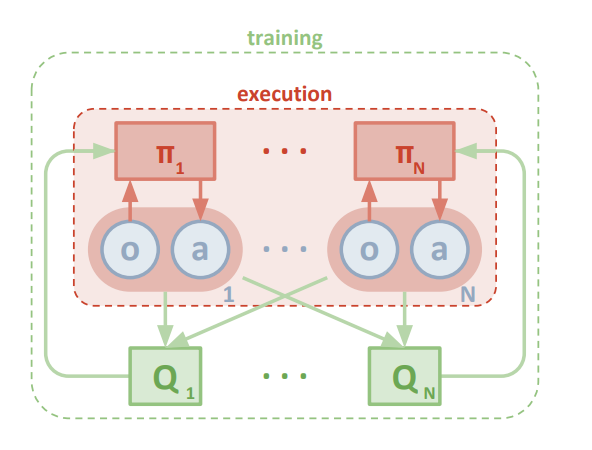
\includegraphics[width = 0.5\hsize]{./figures/MADDPG.png} 
		\caption{MADPGG: multi-agent decentralized actors and centralized critics approach(from \citep{lowe2017multi})} % caption of the figure
		\label{fig:madpgg_architecture} % a label. When we refer to this label from the text, the figure %number is included automatically
	\end{center}
\end{figure}

\subsection{The Actor Network}

The actor network, as shown in Figure \ref{fig:actor_architecture} consists of the following:
	\begin{itemize}
		\item Input layer: The input to the network are the states of the environments observable by the \textbf{individual} agent.
		\item Hidden layer: The two hidden layers are made up of 512 and 256 neuron units respectively with exponential linear units.
		\item Output layer: The network outputs the action taken by the agent, which consists of 2 numbers
	\end{itemize}

\begin{figure}[H]
	\begin{center}
		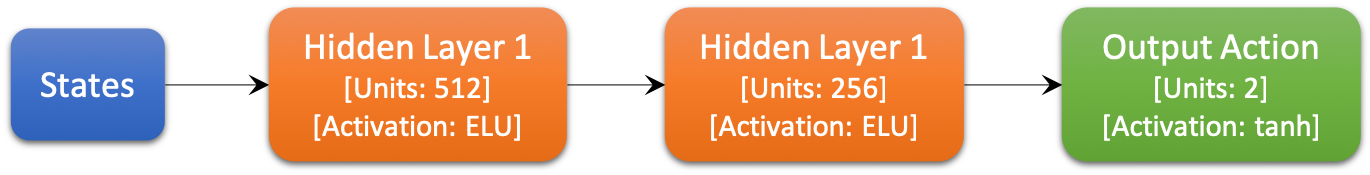
\includegraphics[width = 1.0\hsize]{./figures/Actor.png} 
		\caption{Architecture of the actor network.} % caption of the figure
		\label{fig:actor_architecture} % a label. When we refer to this label from the text, the figure %number is included automatically
	\end{center}
\end{figure}

\subsection{The Critic Network}

The critic network, as shown in Figure \ref{fig:critic_architecture} consists of the following:
	\begin{itemize}
		\item Input layer: The input to the network are the states of the environments observable by the agents.
		\item Hidden layer: Hidden layer 1 takes in the states observable by the agent as input. Hidden layer 2 takes both the output from hidden layer 1 and the action as inputs. Hidden layer 3 takes the output of hidden layer 2 as input.
		\item Output layer: The network outputs the value function of the state-action input.
	\end{itemize}
	
\begin{figure}[H]
	\begin{center}
		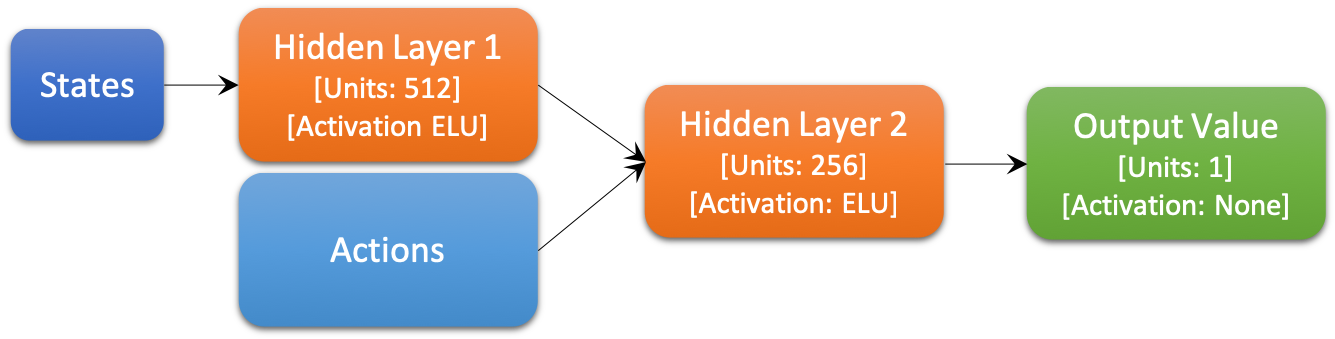
\includegraphics[width = 1\hsize]{./figures/Critic.png} 
		\caption{Architecture of the critic network.} % caption of the figure
		\label{fig:critic_architecture} % a label. When we refer to this label from the text, the figure %number is included automatically
	\end{center}
\end{figure}

While in \citep{lillicrap2015continuous}, the authors mentioned the application of batch normalization with ReLU activation functions for their actor-critic networks. From my experience in Project 2, I found that the training process is more stable by using exponential linear units (ELUs) introduced by \cite{clevert2015fast}. The ELUs retain most of the characteristics of ReLUs but they have an implicit regularization effect which made training much more stable.

\section{Hyperparameters}
The hyperparameters used in training the MADDPG algorithm are listed below:
\begin{center}
	\begin{tabular}{|l|l|}
	\hline
		\textbf{Hyperparameter}							& \textbf{Value}\\\hline
		Actor learning rate, $\alpha^\mu$				& 0.00015 \\
		Critic learning rate, $\alpha^Q$					& 0.00100 \\
		Discount factor, $\gamma$						& 0.99500 \\
		Buffer size												& 150,000\\
		Minibatch size											& 256\\
		Soft update weights, $\tau$						& 0.0020\\
		Update frequency										& Every 1 time step\\
		Number of updates									& 1 update\\
		Initial weight for noise								& 1.0\\
		Noise weight decay									& 0.999990\\
		Long term mean for noise, $\mu_{ou}$		& 0.00\\
		Mean reversion rate for noise, $\theta_{ou}$	& 0.15\\
		Volatility for noise, $\sigma_{ou}$				& 0.25\\\hline
	\end{tabular}
\end{center}

\section{Results}
	
The average rewards during the training process is shown in Figure \ref{fig:results}. The MADDPG algorithm achieves a mean score of 1.50  (exceeding the required 0.50), across 100 episodes after 2800 episodes. 
	
\begin{figure}[H]
	\begin{center}
		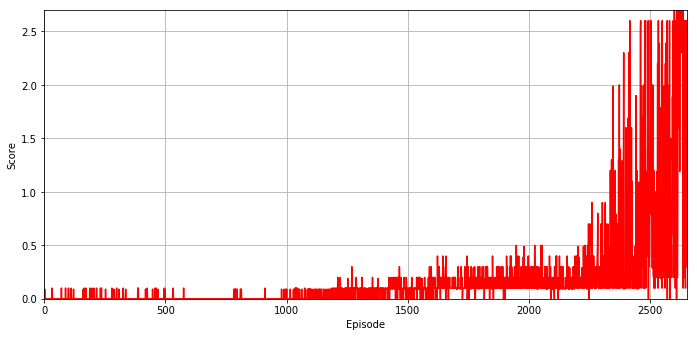
\includegraphics[width = 0.8\hsize]{./figures/results.png} 
		\caption{Average reward vs number of episodes} % caption of the figure
		\label{fig:results} % a label. When we refer to this label from the text, the figure %number is included automatically
	\end{center}
\end{figure}


\section{Ideas for Future Work}
The solution of the problem can potentially improved by applying different algorithms within the multi-agent reinforcement learning framework. It is possible to replace each individual agents with a different algorithm such as A3C and PPOs.\\

Also, a more interesting future work to be done is to deploy the multi-agent deep reinforcement learning in a pure competitive or collaborative game play. The initial intuition is that there is a need for an overall loss function across agents that consists of competing objectives (in a similar fashion as the generative adversarial networks, in which the loss function expresses the competition between the discriminator and the generator).


\section*{Appendix: Deep Deterministic Policy Gradient} \label{appendix}
DDPG, as introduced by \cite{lillicrap2015continuous}, was use to solve this problem. The pseudo-code for DDPG is given in Algorithm 1. The action-value function describes the expected return after taking an action $a_t$ in state $s_t$ and thereafter following policy $\pi$:
\begin{align*}
	Q^\pi(s_t,a_t)	& = \mathbb{E}_{\pi}\left[R_t \vert s_t, a_t\right]\\
						& = \mathbb{E}_{\pi}\left[\sum_{i=t}^T \gamma^{i-t}r(s_i,a_i)\vert s_t, a_t\right]\\
\end{align*}

The action-value function follows the Bellman equation:
\begin{align*}
	Q^\pi(s_t,a_t) &=  \mathbb{E}_\pi\left[r(s_t,a_t) + \gamma \mathbb{E}_\pi\left[Q^\pi(s_{t+1}, a_{t+1})\right] \right]
\end{align*}

Given that the target policy is deterministic, we can described it as $\mu: \mathcal{S} \rightarrow \mathcal{A}$
\begin{align*}
	Q^\mu(s_t,a_t) &=  \mathbb{E}_\pi\left[r(s_t,a_t) + \gamma Q^\mu(s_{t+1}, \mu(s_{t+1})) \right]
\end{align*}



In DDPG, we use non-linear function approximator to learn both the $Q(s_t, a_t)$ action-value function and the policy $\mu(s_t)$.  Firstly, the action-value function is learned using Q-learning, whereby $\mu(s_t) = \text{arg max}_{a\in \mathcal{A}} Q(s_t,a_t)$. Similar to the DQN algorithm introduced by \cite{mnih2015human}, the action-value function $Q(s_t, a_t)$ is learned by minimizing the following loss function:
\begin{align*}
	L(\theta^Q) = \mathbb{E}_{\pi^\prime}\left[(Q(s_t,a_t)-y_t)^2\right]
\end{align*}
where
\begin{align*}
	y_t = r(s_t,a_t) + \gamma Q(s_{t+1}, \mu(s_{t+1})\vert \theta^Q)
\end{align*}

Secondly, the actor network is learned by using the DPG algorithm introduced by \cite{silver2014deterministic}. The actor is updated by the following:
\begin{align*}
	\nabla_{\theta^\mu} J & \approx \mathbb{E}_{\pi^\prime}\left[\nabla_{\theta^\mu}Q(s,a\vert \theta^Q)\vert_{s=s_t, a=\mu(s_t\vert\theta^\mu)}\right]\\
	& = \mathbb{E}_{\pi^\prime}\left[\nabla_a Q(s,a\vert \theta^Q)\vert_{s=s_t, a=\mu(s_t)}\nabla_{\theta^\mu} \mu(s\vert \theta^\mu)\vert_{s=s_t}\right]\\
\end{align*}

One final issue on DDPG is exploration. Exploration is introduced to the algorithm by including some noise in the action.
\begin{align*}
	a_t = \mu(s_t\vert \theta^\mu) + \mathcal{N_t}.
\end{align*}

$\mathcal{N}_t $ is an Ornstein-Uhlenbeck process
\begin{align*}
	d\mathcal{N}_t = \theta_{ou}(\mu_{ou} - \mathcal{N}_t)dt + \sigma_{ou} dW_t
\end{align*}
where
$\theta_{ou}$ is the mean-reversion rate, $\mu_{ou}$ is the long-term mean, $sigma_{ou}$ is the volatility and  $W_t$ is a Brownian motion.


\newpage

\begin{algorithm}[H]
\SetAlgoLined
\textbf{Initialization:}\\
Randomly initialize critic network $Q\left(s,a \vert \theta^Q\right)$ and actor $\mu\left(s\vert \theta^\mu\right)$ with weights $\theta^Q$ and $\theta^\mu$.\\
Initialize target network $Q^\prime$ and $\mu^\prime$ with weights $\theta^{Q^\prime} \leftarrow \theta^Q$ and $\theta^{\mu^\prime} \leftarrow \theta^\mu$.\\
Initialize replay buffer $R$.\\
\;
\For{episode = 1:M}{
	Initialize a random process $\mathcal{N}$ for action exploration.\\
	Receive initial observation state $s_1$.\\
	\;
	\For{t=1:T}{
		Selection action $a_t = \mu(s_t\vert \theta^\mu) + \mathcal{N}$ according to the current policy and exploration noise.\\
		Execute action $a_t$ and observe reward $r_t$ and observer new state $s_{t+1}$.\\
		Store transition $(s_t, a_t, r_t, s_{t+1})$ in $R$.\\
		Sample a random minibatch of $N$ transitions $(s_i, a_i, r_i, s_{i+1})$ from $R$.\\
		Set $y_i = r_i + \gamma Q^\prime(s_{t+1},  \mu^\prime(s_{i+1}\vert \theta^{\mu^\prime})\vert \theta^{Q^\prime})$.\\
		Update the critic network by minimizing:
		\begin{align*}
			L = \frac{1}{N} \sum_i \left(y_i - Q(s_i, a_i\vert \theta^Q)\right)^2.
		\end{align*}
		Update the actor policy using the sampled policy gradient:
		\begin{align*}
			\nabla_{\theta^\mu} J \approx \frac{1}{N} \sum_i \nabla_a Q(s,a\vert\theta^Q) \vert_{s=s_i, a=\mu(s_i)}\nabla_{\theta^\mu} \mu(s\vert\theta^\mu)\vert_{s_i}.
		\end{align*}
		Update the target networks:
		\begin{align*}
			\theta^{Q^\prime} & \leftarrow \tau \theta^Q + (1-\tau)\theta^{Q^\prime} \\
			\theta^{\mu^\prime} & \leftarrow \tau \theta^\mu + (1-\tau)\theta^{\mu^\prime} \\
		\end{align*}
	}	
}

 \caption{Deep Deterministic Policy Gradient (DDPG)}
\end{algorithm}


\newpage

\bibliography{reference}
\bibliographystyle{apalike}


\end{document}
%%% Local Variables: 
%%% mode: latex
%%% TeX-master: t
%%% End: 
